% Options for packages loaded elsewhere
\PassOptionsToPackage{unicode}{hyperref}
\PassOptionsToPackage{hyphens}{url}
%
\documentclass[
]{article}
\usepackage{amsmath,amssymb}
\usepackage{lmodern}
\usepackage{iftex}
\ifPDFTeX
  \usepackage[T1]{fontenc}
  \usepackage[utf8]{inputenc}
  \usepackage{textcomp} % provide euro and other symbols
\else % if luatex or xetex
  \usepackage{unicode-math}
  \defaultfontfeatures{Scale=MatchLowercase}
  \defaultfontfeatures[\rmfamily]{Ligatures=TeX,Scale=1}
\fi
% Use upquote if available, for straight quotes in verbatim environments
\IfFileExists{upquote.sty}{\usepackage{upquote}}{}
\IfFileExists{microtype.sty}{% use microtype if available
  \usepackage[]{microtype}
  \UseMicrotypeSet[protrusion]{basicmath} % disable protrusion for tt fonts
}{}
\makeatletter
\@ifundefined{KOMAClassName}{% if non-KOMA class
  \IfFileExists{parskip.sty}{%
    \usepackage{parskip}
  }{% else
    \setlength{\parindent}{0pt}
    \setlength{\parskip}{6pt plus 2pt minus 1pt}}
}{% if KOMA class
  \KOMAoptions{parskip=half}}
\makeatother
\usepackage{xcolor}
\IfFileExists{xurl.sty}{\usepackage{xurl}}{} % add URL line breaks if available
\IfFileExists{bookmark.sty}{\usepackage{bookmark}}{\usepackage{hyperref}}
\hypersetup{
  hidelinks,
  pdfcreator={LaTeX via pandoc}}
\urlstyle{same} % disable monospaced font for URLs
\usepackage[left=1.5cm,right=1.5cm,top=1.5cm,bottom=1.5cm]{geometry}
\usepackage{longtable,booktabs,array}
\usepackage{calc} % for calculating minipage widths
% Correct order of tables after \paragraph or \subparagraph
\usepackage{etoolbox}
\makeatletter
\patchcmd\longtable{\par}{\if@noskipsec\mbox{}\fi\par}{}{}
\makeatother
% Allow footnotes in longtable head/foot
\IfFileExists{footnotehyper.sty}{\usepackage{footnotehyper}}{\usepackage{footnote}}
\makesavenoteenv{longtable}
\usepackage{graphicx}
\makeatletter
\def\maxwidth{\ifdim\Gin@nat@width>\linewidth\linewidth\else\Gin@nat@width\fi}
\def\maxheight{\ifdim\Gin@nat@height>\textheight\textheight\else\Gin@nat@height\fi}
\makeatother
% Scale images if necessary, so that they will not overflow the page
% margins by default, and it is still possible to overwrite the defaults
% using explicit options in \includegraphics[width, height, ...]{}
\setkeys{Gin}{width=\maxwidth,height=\maxheight,keepaspectratio}
% Set default figure placement to htbp
\makeatletter
\def\fps@figure{htbp}
\makeatother
\setlength{\emergencystretch}{3em} % prevent overfull lines
\providecommand{\tightlist}{%
  \setlength{\itemsep}{0pt}\setlength{\parskip}{0pt}}
\setcounter{secnumdepth}{5}
\usepackage[font={small,it}, labelfont={bf}]{caption}
\usepackage{float}
\floatplacement{figure}{H}
\usepackage{caption}
\captionsetup[figure]{font=footnotesize}
\ifLuaTeX
  \usepackage{selnolig}  % disable illegal ligatures
\fi

\author{}
\date{\vspace{-2.5em}}

\begin{document}

{
\setcounter{tocdepth}{2}
\tableofcontents
}
\thispagestyle{empty}
\hrule
\vspace{0.3cm}
\begin{center}
    \vspace{1cm}
  \huge
    \begin{tabular}[c]{l}
    \\
    Final Report - Datascience MoBi 2022\\
    \\
    \\
  \textbf{Gaining insight on human early organogenesis}\\
  \textbf{through TRA expression analysis}\\
    \\
    Topic 04 - Team 01\\
    \\
  Paul Christmann, Joshua Eigenmann,\\ David Jewanski, Verena Merke \\
  \\
  \\
  \\
  \Large Date:\\
  \Large June 17, 2022\\
  \\
  \\
    \large Supervisor:
    \large Dr. Maria Dinkelacker \\
    \\
    \large Tutor:
    \large Ian Fichter \\
    \\
    \\
    \large Institute of Pharmacy and Molecular Biotechnology\\
    \large Heidelberg University 
    \vspace{0.3cm} \\
    \end{tabular}
    \end{center}

\begin{center}\rule{0.5\linewidth}{0.5pt}\end{center}

\newpage

\hypertarget{abstract}{%
\section{Abstract}\label{abstract}}

A single cell turns into a complex multicellular organism during embryogenesis. While the morphological steps behind this process are mostly understood, the role of molecular pathways as well as transcriptional regulation in embryonic development is still a topic of research. Tissue restricted antigens (TRAs) may be a key to understanding the relation between molecular biological cause and morphological consequence. Since TRA expression is specific to their relative tissue, we attempted to draw conclusions about organ development from TRA expression patterns between week 4 and 9 of embryogenesis. Using microarray data from Yi H \emph{et al.} (2010), we created a dataset of differentially expressed transcripts through limma analysis that includes genes not found by Yi H \emph{et al.}. Based on these data, we could successfully link developmental steps to TRA expression patterns for some of the analyzed organs. Furthermore, we found individual genes associated with processes in neurogenesis. Finally, we attempted without success to define specific TRAs as biomarkers for organogenesis.

\newpage

\hypertarget{introduction}{%
\section{Introduction}\label{introduction}}

\hypertarget{intro-tra}{%
\subsection{TRAs as a tool to gain insight into embryonic development}\label{intro-tra}}

Tissues restricted antigens (TRAs) are originally a concept from immunology. There, they are sets of genes for auto-antigens that enable e negative selection in the thymus, which prevents autoimmune reactions. These TRAs are ordered in clusters and controlled by autoimmune regulator (AIRE) in the medullary epithelial cells (mTECs) and represent the diversity of antigens in the different tissues of an organism (Dinkelacker 2019; Murphy \& Weaver 2018). For aur research, we use a broader definition. Here,TRAs are genes, which are expressed more than 5 times the median in less than 5 different tissues (Dinkelacker, 2019). In contrast to housekeeping genes, this makes TRAs highly specific for individual tissues. Therefore, the existence and functionally of an organ should be correlated with the expression of its associated TRAs. We will use this connection to gain insight into organ development based on gene expression data between week 4 and 9 of embryogenesis.

\hypertarget{intro-tissues}{%
\subsection{Embryonic development during the observed timeframe}\label{intro-tissues}}

In order to compare the results based on expression patterns, it is essential to give an overview about organogenesis during this time. As they are the focus of our research, we will summarize the developments in a few important organs: the liver, testes, spleen, heart, stomach, skin, skeletal muscles and brain.\\
First, the liver sprout begins to form in week 3 after gestation. From week 4, it develops hepatocyte precursors and is innervated by veins. Between week 5 to 9, the production of gallic acid starts. Furthermore, glycogen granules develop by week 8 and glycogen synthesis starts in the following week (Deutsch 2013).\\
The testes initially develop as non sex-specific gonads. At week 5, the first germ cells appear in the gonades. The gender-specific development into ovaries and testes occurs first by week 7 (Benninghoff 1993).\\
The spleen appears at week 6 of embryonic development. Blood vessels in the organ develop from week 8 to 9 (James \& Jones 1983). Especially important is the spleen's role in the human immune system. To that end, B-lymphocytes are present within this tissue from week 12, while T-cells can be found not earlier than week 14. Previously, these cells develop in the liver starting week 9 and in the thymus from week 7 respectively (Hayward 1983).\\
At week 3, the heart consists only of a preliminary tube. From then on, it undergoes extensive growth and development with cambers and ventricles forming. The fundamental layout is already present by week 5. Then, further remodeling takes place until around week 7, at which point the major steps are already completed (Ulfig 2009; Hikspoors \emph{et al.} 2022).\\
The stomach develops from the foregut. The primitive gut divides into foregut, midgut and hindgut by week 4. At the end of that week, the stomach is first visible (Kluth \emph{et al.} 2013). Gastric pits form by week 8, while most essential cell types (enteroendocrine cells, mucous cells) appear between the 10th and 15th week and stomach acid is only secreted from week 32 onward (Esrefoglu \emph{et al.} 2017).\\
Skin development starts immediately after gastrulation at week 3. The ectoderm further develops to the nervous system and skin epithelium. There, the epidermal differentiation is illustrated through the expression of keratin genes. Adhered cells (periderm) create a protective layer for the ectoderm during weeks 4 to 8 (Hu \emph{et al.} 2018).\\
The skeletal muscles from mesoderm first in form of myoblasts that later (between week 10 and 13) fuse to form myotubes and then differentiated muscle fibers. The proteins necessary for muscle formation appear the earliest at 7 weeks, with more being expressed from week 9 and 10. Muscle fibers only form from week 15 onwards (Romero \emph{et al.}. 2013).\\
With neurulation happening around week 4, the major parts of the brain are already visible by week 9. Between theses stages, characteristic steps of neuronal development such as neuronal proliferation and differentiation (starting at week 4) as well as neuronal migration and synapse formation (starting at week 9) a take place (National Research Council and Institute of Medicine 2009; Müller \& Hassel 2018)). These processes are influenced through signals provided for instance by chemokines.

\hypertarget{intro-brain}{%
\subsection{Chemokines and brain development}\label{intro-brain}}

Chemokines are a group of small proteins, acting as chemoattractors on effector cells. They are classified in 4 groups (alpha to delta), depending on the position of their first cysteines (C). In the alpha group (or CXC), they are separated by a single aminoacid. In the beta group (or CC), they are next to each other. In the gamma group (or C), there is only one cystein present. In the delta group (or CX3C), they are separated by three aminoacids. (Yusuf \emph{et al.} 2005). Chemokines induce cell migration by binding to their respective receptors (a G-Protein coupled receptor), which are often shortened with an R. For example CXCR4, the receptor of the alpha class ligand CXCL12. The function of chemokines during embryonic development is a target of further research. Nevertheless, the CXCL12/CXCR4 signalling pathway plays an important role in the neuronal cell migration (Tiveron \& Cremer 2008).

\hypertarget{methods}{%
\section{Methods}\label{methods}}

\hypertarget{programming-language-and-libraries}{%
\subsection{Programming language and Libraries}\label{programming-language-and-libraries}}

We used the programming language R version 4.2.0 and its IDE RStudio to draw statistical conclusions. We installed the library packages (Table 1) from CRAN and bioconductor, which an open software library statistical genomics. Annotation packages for microarrays were provided by brainarray.

\begin{table}[htb]
\caption{All libraries used for the code of this report, libraries installed from CRAN, Bioconductor and brainarray}
\resizebox{\textwidth}{!}{
\begin{tabular}{@{}ll|ll|ll|ll@{}}
\toprule
\textbf{Library}       & \textbf{Version} & \textbf{Library} & \textbf{Version} & \textbf{Library} & \textbf{Version} & \textbf{Library}     & \textbf{Version} \\ \midrule
affy                   & 1.74             & AnnotationDbi    & 1.58             & biomaRt          & 2.52             & cluster              & 2.1.3            \\
clusterProfiler        & 4.4.4            & cowplot          & 1.1.1            & dplyr            & 1.0.9            & enrichplot           & 1.16.1           \\
factoextra             & 1.0.7            & ggbiplot         & 0.55             & ggforce          & 0.3.3            & GGally               & 2.1.2            \\
ggplot2                & 3.3.6            & ggplotify        & 0.1.0            & ggpubr           & 0.4.0            & ggrepel              & 0.9.1            \\
ggsci                  & 2.9              & ggupset          & 0.3.0            & grid             & 4.2.0            & gridExtra            & 2.3              \\
gt                     & 0.6.0            & gtExtras         & 0.4.1            & hexbin           & 1.28.2           & hgu133plus2hsenstcdf & 25.0             \\
hgu133plus2hsenstprobe & 25.0             & igraph           & 1.3.2            & kableExtra       & 1.3.4            & limma                & 3.52             \\
magick                 & 2.7.3            & magrittr         & 2.0.3            & org.Hs.eg.db     & 3.15             & pheatmap             & 1.0.12           \\
png                    & 0.7              & Rcpp             & 1.0.9            & RCurl            & 1.98             & readxl               & 1.4              \\
rentrez                & 1.2.3            & Rfssa            & 2.0.1            & stringr          & 1.4              & svglite              & 2.1              \\
tidyverse              & 1.3.1            & treemapify       & 2.5.5            & VennDiagram      & 1.7.3            & viridis              & 0.6.2            \\
vsn                    & 3.64             & webshot          & 0.5.3            & XML              & 3.99             &                      &                  \\ \bottomrule
\end{tabular}}
\end{table}

\hypertarget{dataset}{%
\subsection{Dataset}\label{dataset}}

We obtained the data set from Yi H \emph{et al.} (2010). It contains human embryonic data, which covers every week between the 4th and 9th week with three replica at each point in time, hence the data from 18 embryos were acquired. The timezone covers the Carnegie stages 10-23, finishing the process of embryogenesis and organogenesis. This peroid of embryogenesis is highly regulated with considerable differential gene expression. Overall, the data set suits the requirements for our purpose.

\hypertarget{affymetrix-u133-plus-2.0-human-genechip-array-and-importing-its-data}{%
\subsubsection{Affymetrix U133 plus 2.0 human GeneChip array and importing its data}\label{affymetrix-u133-plus-2.0-human-genechip-array-and-importing-its-data}}

The data was generated using Affymetrix U133 plus 2.0 human GeneChip arrays, coted slides with matrices for screening purposes. \href{https://www.affymetrix.com/support/technical/datasheets/human_datasheet.pdf}{The HG-U133 Plus 2.0} allows the detection of about 50,000 transcripts and include 62 control transcripts.

We downloaded the raw data from the Gene Expression Omnibus with the Accession Number of \href{https://www.ncbi.nlm.nih.gov/geo/query/acc.cgi?acc=GSE15744}{GSE15744}. We imported it with the library package \emph{affy}, which allows more manageable data analysis and manipulation of microarray intensity values.

To access the data remotely, we uploaded it to the cloud-based repository hosting service github. It can be imported with the library \emph{Rfssa}.

\hypertarget{quality-control-of-the-suface-images-and-of-rna-degradation}{%
\subsubsection{Quality control of the suface images and of RNA Degradation}\label{quality-control-of-the-suface-images-and-of-rna-degradation}}

As shown in Figure \ref{fig:QC-surface-images-and-RNA-Degradation-Plot}A the surface of the microarrays show no spatial artefacts, fingerprints, irregular dye or stripes. Some differences in overall brightness are visible but marginal.

Furthermore, we tested for low RNA quality chips. Coted matrices degrade under unfavorable conditions, which negatively affects raw intensities (Fasold \& Binder 2013). By plotting the RNA degradation for 3'--5' strand, we compare the different chips (Figure \ref{fig:QC-surface-images-and-RNA-Degradation-Plot}B) and verify the overall chip quality for data analysis.

\begin{figure}
\centering
\includegraphics{final_report_files/figure-latex/QC-surface-images-and-RNA-Degradation-Plot-1.pdf}
\caption{\label{fig:QC-surface-images-and-RNA-Degradation-Plot}\textbf{Quality control: Selected surface image of a microarray shows no damage or artefacts and RNA degradation plot shows slight irregularities and verifies the data.} \textbf{A}: The microarray inspection shows no irregularities and every chip is accepted for further data analysis. \textbf{B}: Some crossing lines can be seen, especally the microarray GSM394519. We decided that the inconsistencies are minor though, and kept all microarrays to avoid the loss of potentionally relevant data.}
\end{figure}

\hypertarget{normalising-the-data-set}{%
\subsection{Normalising the data set}\label{normalising-the-data-set}}

Intensity values of different chips are affected by statistical variance and random fluctuation. To access the biological relevant variation, the raw data is normalised. We chose the vsn rma normalization with its library \emph{vsn} according to Huber \emph{et al.} (2002). This library is designed to process microarray intensity values. It calibrates data and applies \emph{generalized log}-transformation, which is an adjusted natural logarithm and preserves statistical significance.

\hypertarget{QC-normalization}{%
\subsubsection{Quality control of the vsn normalization}\label{QC-normalization}}

To verify the transformed data intensity values, some test can be performed (supplementary Figure \ref{fig:QC-normalization-plots}). After the normalization, the rank of the mean of the intensity values and their standard deviation should not correlate. To control this, we plotted the rank of the mean against the standard deviation, which resulted in a reasonable horizontal line indicated in red (supplementary Figure \ref{fig:QC-normalization-plots}A).~To further control the normalization we visualized the intensity values. We used boxplots to compare each of the 18 microarray separately by its mean, median and variance (supplementary Figure \ref{fig:QC-normalization-plots}B). We deduced that all arrays fit.. The second option gives us the ability to zoom in even further. The intensity levels of three replica should be the same, since they were taken at the same time. We can use scatterplots to compare single intensity levels. With one of the replica applied on the x and y axis respectively, we should see a scatterplot following the linear function y = x since the same transcript should show the same intensity in both replica (supplementary Figure \ref{fig:QC-normalization-plots}C).

\hypertarget{analytical-methods}{%
\subsection{Analytical methods}\label{analytical-methods}}

\begin{enumerate}
\def\labelenumi{\arabic{enumi}.}
\item
  Annotation
  To make sense out of the intensity values they need to be associated to common data with known properties. We applied the data frame \emph{ensembl\_103.txt} provided by Dr.~Dinkelacker, to annotate our data and yield the appropriate transcript ID for the Probe ID of the microarray. To annotate for TRAs, we applied another data frame by Dr Dinkelacker called \emph{tra.2017.human.gtex.5x.table.tsv}.
\item
  Limma
  The \emph{limma} package determines among many other things the changes of gene expression over time in intensity values of microarrays. It facilitates advanced statistical algorithms to calculate the necessary coefficients of a linear model for every intensity value in the data set. It uses information borrowing, quantitative weighting, variance modelling and data preprocessing, while not subset the data (Ritchie. \emph{et al.} 2015). Because the linear model was casted on every intensity value, statistical tests called Empirical Bayes can determine differential expressed genes via t-statistics and their associated p-values.
\item
  Over representation analysis
  The statistical method over-representation analysis determines among other thing the over represented function of genes with associated transcripts in a subset of a mother data set with annotated transcripts and known functions. Categories for functions can be accessed via gene ontology.
\end{enumerate}

\hypertarget{results}{%
\section{Results}\label{results}}

\hypertarget{limma}{%
\subsection{Limma analysis}\label{limma}}

To filter our data for biological interesting data, we performed \emph{limma} analysis to extract differentially expressed genes. Our threshold for significance is an Benjamini-Hochberg adjusted p-value of 0.01 or below. We found changes of gene expression in 1,814 transcripts.

The gathered dataset from limma analysis of the differential expression between weeks 4 to 9 was used to created a volcano plot. The negativ log10 of the adjusted P-value was ploted against the logFC value. The -log10 (adjusted P-value) boundary was set at 2 which equals our targeted adjusted P-value of 0.01. The logFC boundarys were -1 and 1, which reflects a doubling in the expression (Supplementary: Figure \ref{fig:Volcano-Plot}). The genes were categorized in two groups:

\begin{enumerate}
\def\labelenumi{\arabic{enumi}.}
\tightlist
\item
  up-regulated if the logFC value is larger than 1 and the adjusted P-value is smaller than 0.01
\item
  down-regulated if the logFC value is smaller than 1 and the adjusted P-value is smaller than 0.01
\end{enumerate}

Genes which didn't belong in those groups were declared as not differentially expressed. The differentially expressed genes between all weeks with an adjusted P-value smaller then 0.01 were further used.

\hypertarget{paper-comp}{%
\subsection{Comparison of differential expressed genes between the original paper and our method}\label{paper-comp}}

We acquired the data from the original paper from the supplemental materials. We imported it into a data frame annotated it with the use of our data set because the both have the same probe set IDs from the same microarray.

\hypertarget{venn-diagram}{%
\subsubsection{Venn diagram}\label{venn-diagram}}

To determine the number of transcripts which overlap between the data of the paper and our data, we plotted a Venn diagram (Figure \ref{fig:Venn-Diagram}).

The intersection showed a number of transcripts worth for further analysis.

\hypertarget{verifing-the-trends-postulated-in-the-paper-with-our-data}{%
\subsubsection{Verifing the trends postulated in the paper with our data}\label{verifing-the-trends-postulated-in-the-paper-with-our-data}}

In contrast to our method using limma, the authors of the original paper used \emph{One-way analysis of variance} with a p-value of 0.05 to determine the differential expressed genes (Yi H \emph{et. al}, 2010). In the paper they provided an annotation of transcripts that were regulated \emph{up}, \emph{down} or showed an \emph{arch}. We used k-means clustering to determine, if we see these trends in our data aswell (Figure \ref{fig:paper-trends-cluster}).

\begin{figure}
\centering
\includegraphics{final_report_files/figure-latex/paper-trends-cluster-1.pdf}
\caption{\label{fig:paper-trends-cluster}\textbf{Clustering of the common transcripts reveals similar trends and but our additional data shows missing differentially expressed genes.} We chose data with transcript IDs both in the data set of the original paper and in our TRA data. Additionally they had to be annotated as \emph{up, }down\emph{, or }arch* by the authors of the paper. The \emph{up} and \emph{down} regulated transcript-data (\textbf{A} and \textbf{B}) follow the same pattern as postulated in the paper. For the \emph{arch} regulated transcript-data (\textbf{C}) we see clusters, with same matching the \emph{arch} pattern and some who are rather undetermined. Of 396 transcripts only 39 of our differentially expressed genes by \emph{limma} analyis share this \emph{arch} property (\textbf{D}). Here we clearly see differential gene expression. In \textbf{E} we plotted data of our differntially expressed genes. There are \emph{up} and \emph{down} regulated genes determined by our \emph{limma} analysis, that are not included in the data set of the authors of the original paper}
\end{figure}

We repeated the Figure\ref{fig:paper-trends-cluster}A and B with our differentially expressed genes as well and the results were highly similar. The Figure can be found on our github (Report/Comparison with paper differentially expressed.png).

For Figure \ref{fig:paper-trends-cluster}C cluster 1, 6, 7, 8 clearly show an \emph{arch} regulated pattern, but for clusters 4 and 5 the data rather appears to be \emph{down} regulated, or \emph{up} regulated in the case of cluster 10. And the final clusters 2, 3 and 9 with a total of 156 transcripts are not differentially expressed at all. When we cluster our differentially expressed genes annotated with the \emph{arch} pattern (Figure \ref{fig:paper-trends-cluster}D), we recieve only 10\% of the amount of transcripts which are clearly clusters.

Figure \ref{fig:paper-trends-cluster}E reveals, that there clearly \emph{up} and \emph{down} regulated genes of 646 transcripts or about 10\%, that are missed by the method used by the authors of the paper.

\hypertarget{organ}{%
\subsection{TRAs can infer a basic timeline of organ development}\label{organ}}

\hypertarget{organ-overview}{%
\subsubsection{Differentially expressed transcripts can be linked to all analyzed tissues}\label{organ-overview}}

\begin{figure}
\centering
\includegraphics{final_report_files/figure-latex/unnamed-chunk-6-1.pdf}
\caption{\label{fig:unnamed-chunk-6}A. The number of transcripts associated with each tissue, including subtissues, is displayed. B. The plot shows the share of TRAs associated with each tissue. Subtissues are subsumed under their main tissue.}
\end{figure}

The TRA dataset covers 53 distinct tissues. For all of those, we found at least 40 differentially expressed transcripts within our dataset. The minimum were 46 stomach-linked transcripts, the highest reached 837 TRAs for the testes.These numbers are sufficient for further analysis of the gene expression within individual tissues. Therefore, all results will be based on our dataset with differentially expressed genes from limma analysis.\\
Nonetheless, it should be noted that there is a significant overlap between the TRAs associated with different tissues, especially as each transcript is on average linked to 7.4 different sub-tissues or tissues. This overlap is illustrated by supplementary Fig. \ref{fig:tissue-links}. Furthermore, a detailed heatmap for the shared TRAs between tissues is shown in the supplementary Fig. \ref{fig:heatmap-tissues}.

\hypertarget{organ-cluster}{%
\subsubsection{The expression of all TRAs associated with a tissue cannot be used to infer organ development}\label{organ-cluster}}

In this research, we attempt to draw conclusions about the developmental state of a tissue based on the expression of genes associated with it alone. For all differencially expressed transcripts associated with one tissue, we analyzed the share of transcripts above a certain expression level over time, as shown in Fig. \ref{fig:expression-plot}A. Furthermore, we observed trends within the median expression of these trascnrips (Fig. \ref{fig:expression-plot}B). Since both metrics only depicted miniscule changes, we hypothesized that distinct, counteracting trends in expression exist within one tissue. Thus, k-means clustering was used to determine groups of TRAs with similar expression patterns. For each of these clusters, the median expression was plotted as shown in Fig. \ref{fig:expression-plot}C. The clustering graphs for all tissues can be found on our github repository.

\begin{figure}
\centering
\includegraphics{final_report_files/figure-latex/expression-plot-1.pdf}
\caption{\label{fig:expression-plot}A. For different expression thresholds the share of differentially expressed transcripts with higher expressions than the threshold is depicted. B. The median expression for all spleen-associated TRAs is shown for each point in time. C. For k-means clustring, the silhouette score determined an optimum of two clusters. The median expression analog to B is plottet for each of these clusters.}
\end{figure}

For many tissues, as shown here exemplary with the spleen, the clustering revealed two or more clusters that could be characterized as either an upregulation or a downregulation. In order to determine the indications for organ development, we analyzed the functions of the transcripts belonging to the two clusters.

\hypertarget{organ-tables}{%
\subsubsection{The clusters of up- and downregulated transcripts can be linked to distinct gene functions.}\label{organ-tables}}

As shown in supplementary Fig. \ref{fig:spleen-boxplot}, the spleen is a clear example of two dinstict clusters with one consisting of upregulated previously inactive genes and one with downregulated highly active genes. For all these differentially expressed transcripts, we used the NCBI gene database to get a functional annotation. Of the 98 upregulated genes, 48 had a functional annotation. 17 of those were clearly associated with immune system or blood functions and thus relevant for the functional thymus. We further found 157 downregulated genes. There, 70 were annotated and 45 of those displayed a relation to the cell cycle or cell division. The tables of the transcripts with a relevant function are visible in the suppplementary material (Fig. \ref{fig:spleen-up-table} and Fig. \ref{fig:spleen-down-table}).

\hypertarget{organ-ora}{%
\subsubsection{Overrepresentation Analysis can create plots that signify organ development}\label{organ-ora}}

For this analysis, the eight tissues with the most meaningful results were chosen.In Fig. \ref{fig:ORA-plot}, the most important functions for these tissue were determined through overrepresentation analysis. In addition, the Expression of the associated transcripts was plotted.

\begin{figure}
\centering
\includegraphics{final_report_files/figure-latex/ORA-plot-1.pdf}
\caption{\label{fig:ORA-plot}For eight tissues A to H, the tables show the 10 most significant results from overrepresentation analysis. There, the functional GO annotation of all transcripts in our dataset (not only the differentially expressed ones) was compared to the functions associated with all TRAs of one tissue. The significance was determined by an adjusted p-value. Of those 10 gene sets, up to 5 were chosen to represent different groups of functions and avoid the overlap of highly related processes. For each of those, the median expression for each week was calculated and plotted, as seen in the expression graphs.}
\end{figure}

For the spleen (Fig. \ref{fig:ORA-plot}A), we determined a largely constant expression of immune-related genes throughout the time frame, with a slight increase in some functions from week 7-9.
The brain (Fig. \ref{fig:ORA-plot}B) showed an increase in neuron projection morphogenesis from a previously inactive state (expression \textless{} 6.8) in week 4 to a significant expression (\textgreater7.5) by week 8. Synaptic signaling stayed at relatively constant expression levels.
Heart-associated functions (Fig. \ref{fig:ORA-plot}C) can be grouped into two categories. Cardiac functions (cardiac muscle tissue development, heart contraction) are highly expressed in week 4 and fall continously until week 8. In contrast, general muscle gene sets are rising from originally lower expression levels during the observed time.
The liver (Fig. \ref{fig:ORA-plot}D) shows no clear expression patterns, with some metabolic functions increasing through time (organic hydroxy compound metabolic process) while others stay mostly constant (cellular amino acid metabolic process) or fall (organic acid catabolic process). In contrast, skeletal muscle gene sets (Fig. \ref{fig:ORA-plot}E) show a very clear trend. After a mostly slight increase between week 4 and 8, a sharp rise in expression levels is visible from week 8 to 9.
The testis-associated sets (Fig. \ref{fig:ORA-plot}F) continuously decrease in expression from week 5 onward.
For the stomach (Fig. \ref{fig:ORA-plot}G), we found a initially high expression in week 4 that then falls until week 6 and then increases again towards week 9.
Finally, the skin-associated functions (Fig. \ref{fig:ORA-plot}H) all displayed a constant rise in expression levels from week 5 to 9.

\hypertarget{brain}{%
\subsection{Hypothesis: Neural TRA expression patterns reflect morphological brain development}\label{brain}}

The annotated dataset after limma analysis was filtered to determine which genes are differentially expressed in a certain tissue. The discovered genes were examined with NCBI to determine their function. The genes of interest are categorized in three groups:

Our data covered 13 different brain subtissues, whose TRAs showed a signficant overlap. Hence, we filtered the differentially expressed transcripts for those that are only related to one of all 13 subtissues. The discovered genes were examined using the NCBI database. The resulting genes of interest can be categorized as follows:\\
1.Genes of Ion channels 2.Genes for neuronal development 3.Genes of cytokines

\begin{figure}
\centering
\includegraphics{final_report_files/figure-latex/gene-expression-brain-1.pdf}
\caption{\label{fig:gene-expression-brain} The gene expression of different transcripts coding for an ion channel (left), neuronal development and function proteins (middle) and chemokine-related genes (right) was plotted for week 4 to 9.}
\end{figure}

\hypertarget{ion-channel}{%
\subsubsection{Ion channel}\label{ion-channel}}

Ion channels play an important role in the function of neurons. We discovered that ENST00000531293 is highly expressed in the nucleus accumbens. It shows a significant increase between weeks 7 to 9 and codes for SLN sarcolipin which is a sarcoplasmic reticulum Ca-ATPase.

\hypertarget{genes-for-neuronal-development-and-function}{%
\subsubsection{Genes for neuronal development and function}\label{genes-for-neuronal-development-and-function}}

The second group are genes with a specific role in neuronal development and function. There, we discovered that ENST00000276646 and ENST00000529690 expression increases significantly over time. Both transcripts are associated with the cerebellar hemisphere and code for SYBU (syntabulin), a protein that contributes to activity-dependent presynaptic assembly in neuronal development.\\
Furthermore, we found four transcripts for axon goudance: ENST00000602349 codes for NXPH1 (neurexophilin 1) which forms a tight complex with neurexins. These proteins promote adhesion between axons and dendrites. The transcript shows a strong rise in expression, especially from weeks 7 to 8, and is connected to the anterior cingulate cortex.\\
ENST00000518312 and ENST00000521485 encode for SNAP91 (synaptosome associated protein 91), which plays a role in regulation of clathrin-dependent endocytosis. Therefore, SNAP91 is important for essential axonal functions of neurons like postsynaptic density (Overhoff et al.~2020). The gene is associated with the cerebellar hemisphere and also shows a significant increase between weeks 7 to 8.\\
In addition, ENST00000539563 encodes for LSAMP (limbic system associated membrane protein) which plays a role in axon guidance. The encoded preprotein is processed into a neuronal surface glycoprotein which functions as an adhesion molecule during axon guidance and neuronal growth in the developing limbic system. ENST00000539563 is associated with the Putamen, a part of the basal ganglia that are associated with the limbic system-
ENST00000356660 and ENST00000439476 code for BDNF (brain derived neurotrophic factor). A binding of BDNF to its receptor promotes neuronal survival. Both transcripts show an identical decline in expression over the weeks. Nonetheless, ENST00000356660 is connected to cerebellar hemisphere while ENST00000439476 to related to the hippocampus.

\hypertarget{chemokine-related-genes}{%
\subsubsection{Chemokine related genes}\label{chemokine-related-genes}}

The last group are chemokines, proteins with an important role in the signaling process during neuronal development (Tiveron 2008). We discovered ENST00000337225, which encodes for CXCL14 (alpha class chemokin ligand). It shows a strong increase in expression between weeks 4 to 6 and is associated with the anterior cingulate cortex. ENST00000579298 encodes for NUP85 (nucleoporin 85), a protein component of the Nup107-160 subunit of the nuclear pore complex. NUP85 can bind to CCR2 (a receptor for beta class chemokines) and promotes the chemotaxis of monocytes. ENST00000579298 is related to the frontal cortex and shows a decline between weeks 5 to 9.

\hypertarget{hypothesis-specific-tras-can-be-used-as-key-biomarkers-for-the-development-of-individual-organs}{%
\subsection{Hypothesis: Specific TRAs can be used as key biomarkers for the development of individual organs}\label{hypothesis-specific-tras-can-be-used-as-key-biomarkers-for-the-development-of-individual-organs}}

\hypertarget{principal-component-analysis}{%
\subsubsection{Principal component analysis}\label{principal-component-analysis}}

Principal component analysis (PCA) was performed on a matrix containing all differentially expressed genes throughout the 6 weeks. This was performed to reduce dimension while keeping most of the data's variance. To get a better grasp of how much variance is explained by each principal component (PC), the percentage variance of each PC together as well as the cumulative variance were plotted. This visualization helps to determine how many PCs are needed to explain a significant amount of the data's variation. The chosen PCs can than be used for further analysis. The first three PCs already explain over 80\% of the data's variance, with the first PC alone accounting for over 60\% (Fig. \ref{fig:PCA-analysis} A).

For further analysis, each transcript was awarded a rank depending on how much it contributes to each PC. Then, a score was calculated for maximum contribution to PC1 and minimal loadings for all other relevant PCs (PC2-5). We took a closer look at the five best socring transcripts for PC1, as this PC alone already explains the brunt of the variance of our data. These transcripts encode for three different proteins: Low-Density Lipoprotein Receptor Class A Domain-Containing Protein 4 (LDLRAD4) encoded by ENST00000399848, Calcium-activated potassium channel subunit beta-2 (KCNMB2) encoded by ENST00000432997 and ENST00000452583 and SLIT And NTRK-Like Protein 3 (SLITRK3) encoded by ENST00000241274 and ENST00000475390.

The transcripts of ENST00000432997 and ENST00000452583 encode for the same Protein (KCNMB2). Fitting to that, both transcripts consistently display the same expression level over all weeks. The same applies to the transcripts of ENST00000241274 and ENST00000475390, as they also encode for the same protein (SLITRK3) and therefore also display the same expression levels. The transcripts for LDLRAD4 show the highest overall expression levels. Their expression pattern also does not display many similarities to those of KCNMB2 and SLITRK3. However, KCNMB2 and SLITRK3 show a highl similar curve over all weeks (Fig. \ref{fig:PCA-analysis} B).

\includegraphics{final_report_files/figure-latex/PCA-analysis-1.pdf}

\hypertarget{discussion}{%
\section{Discussion}\label{discussion}}

\hypertarget{comparison-with-original-paper}{%
\subsubsection{Comparison with original paper}\label{comparison-with-original-paper}}

In contrast to our \emph{limma} analysis to generate data with biological relevance, the authors of the original paper (Yi H \emph{et al.}, 2010) of our data set used \emph{One-way analysis of variance} to acquire differential expressed genes. We compared both data subsets by k-means clustering and plotting the overlapping Intensity values (Figure \ref{fig:paper-trends-cluster}). By looking at the trends of the cluster for \emph{up} and \emph{down} regulated gene expression, we can validate the method used by the authors. In contrast the \emph{arch} regulated genes-clusters do not present a clear result and show a weakness of the method used. It falsely detects some genes as differentially expressed, assuming our \emph{vsn} normalization is correct, which is indicated by the quality control (section \ref{QC-normalization}).\\
Furthermore, we showed in our Venn diagram (Figure \ref{fig:Venn-Diagram}), that our method detected differentially expressed genes not included in their data. This questions the significance of either the papers results or again our \emph{vsn} normalization and subsequent \emph{limma} analysis, which is rather unlikely given our quality control and plots.\\
The discrepancy can be explained by the publication date, which is year 2010. Now there are more advanced algorithms that determine differentially expressed genes more precisely. The \emph{vsn} and the \emph{limma} package are up to date with frequent advances (Ritchie. et al.~2015).\\
Overall, this ensured the quality of our data set and differentially expressed genes while also pointing out some flaws of the data set of the paper.

\hypertarget{dis-organ}{%
\subsubsection{TRAs can infer a basic timeline of organ development}\label{dis-organ}}

In our analysis, we have shown that a number of TRAs are differentially expressed (section \ref{organ-overview}) between week 4 and 9 of human embryonic development in each of the analyzed tissues. Nonetheless, the expression levels of TRAs associated with one tissue do not constitute a useful metric for the organ's development (section \ref{organ-clustering}). This can be explained by the fact that within one tissue's TRAs, there are multiple groups of genes both distinct in expression patterns (clustering in section \ref{organ-clustering}) and function (analysis of spleen gene functions in section \ref{organ-tables}). Thus, we determined that the expression over time of functional gene sets linked to specific tissues through overrepresentation analysis is a more meaningful metric for organ development.

This approach was used in section \ref{organ-ora} for eight different tissues.
For the spleen, the results of our analysis (Fig. \ref{fig:ORA-plot}A) largely do not reflect the embryonic development (section \ref{intro-tissues}). While some of the immune-related gene sets are already expressed in week 4, the spleen only develops in week 6 and contains immune cells by week 12. This shows that while the spleen plays a role in the immune system and such gene sets are therefore rightly linked to the spleen, the expression of these transcripts alone does not necessarily relate to the development of the organ. It is still noteworthy that functions related to the adaptive immune system increase in expression form week 7 onward, which correlates with the beginning of T-cell development in the thymus.\\
The observed timeframe is an important part of brain development (section \ref{intro-tissues}). This is also visible in the expression data (Fig. \ref{fig:ORA-plot}B), with a already high but still continously increasing expression of synaptic gene sets. Furthermore, as the brain starts to form, the expression of neuron projection morphogenesis transcripts increases continuously from week 5 to 8.\\
At week 4, the clearly heart-associated gene sets (Fig. \ref{fig:ORA-plot}C) are at their highest expression level and decrease until week 8. The cardiac muscle tissue development transcripts still remain highly expressed (\textgreater7.5). This corresponds to the early development of the heart as noted in the introduction (section \ref{intro-tissues}). It is noteworthy that the heart contraction gene set rises in expression again from week 8 to 9, but here an explanation is not possible without further analyzing the individual genes.\\
The liver-associated TRAs showed no clear expression pattern (Fig. \ref{fig:ORA-plot}D). Thus, even though the liver forms mostly during the analyzed timeframe (section \ref{intro-tissues}), we cannot link the gene expression to the organ's development. The detected functions are mostly metabolic pathways whose activity could also be related to processes outside the liver. As a result, it is plausible that their expression is independent of liver development.\\
The skeletal muscle functions are expressed only late within the observed time, as shown by the large increase in expression from week 8 to 9 (Fig. \ref{fig:ORA-plot}E). As muscle fibers begin to develop later than week 9 and the first related proteins appear from week 7 on (section \ref{intro-tissues}), these expression data correspond well to the embryonic development.\\
The testis gene sets decrease in expression from week 5 onward (Fig. \ref{fig:ORA-plot}E). This is in contrast to the embryonic development, where the gonads start to form at around the same time (section \ref{intro-tissues}).\\
For the stomach, the expression pattern indicates a decrease until week 6 followed by rising expression levels until week 9 (Fig. \ref{fig:ORA-plot}G). However, the literature indicates that these results are unrelated to the stomach development. Functions like digestion or peptide hormone secretion are impossible to occure at this time, since the specific cells needed for this only appear later in embryogenesis (section \ref{intro-tissues}). Therfore, the cause of the changing expression would have to be determined through a more in-depth analysis of the involved genes.\\
Finally, the skin shows an increased expression of related genes sets from week 5 to 9 (Fig. \ref{fig:ORA-plot}H). This broadly reflects the embryonic development, with the epidermis starting to form in week 4 (section \ref{intro-tissues}). We also found this expression pattern in the keratinization gene set that is suggested by literature as a good indicator for skin formation.

\hypertarget{dis-brain}{%
\subsubsection{Brain subtissue-specific gene expression reflects neuronal development processes}\label{dis-brain}}

First, we found a significant increase in the expression of SLN sarcolipin (a Ca-ATPase) (Fig. \ref{fig:gene-expression-brain} left). Since Ca(2+) is an essential cofactor for actin dependent cell migration, this might be related to neuronal migration startingweek 9 (section \ref{intro-tissues}).\\
Additionally, the strong correlation between the expression of SNAP91 genes and one SYBU gene (ENST00000276646) (Fig. \ref{fig:gene-expression-brain} middle) was noteworthy. Both proteins are associated with the cerebellar hemisphere and contribute to endocytosis (Overhoff et al.~2020).\\
In addition we identified a significant increase in expression of NXPH1 (Fig. \ref{fig:gene-expression-brain} middle). An upregulation of this factor can prepare the process of synapse formation which starts at week 11 (section \ref{intro-tissues}).\\
We further identified a strong LSAMP expression associated to the putamen as well as NXPH1 linked with the anterior cingulate cortex. (Fig. \ref{fig:gene-expression-brain} middle). As adhesion molecules for axon guidance, their increases in expression (from week 6/7 on) could be in preparation for synapse formation at week 9 (section \ref{intro-tissues}).\\
The neuronal cell migration is strongly dependent on chemoattractors like chemokines (Tiveron 2008). We identified a significant increase in CXCL14 between weeks 5 to 6 that maintains a high expression level afterwards. Fig. \ref{fig:gene-expression-brain} right). This could be an accumulation for neuronal migration, starting by week 9 (section \ref{intro-tissues}). A decline in NUP85 expression is also notable (Fig. \ref{fig:gene-expression-brain} right). NUP85 can bind to CCR2, hence a decline in reduce the chances for this binding. A consequence might be that more CCR2 receptors are free for beta type chemokin mediated signals.
Overall, there were two cases were two closely related transcripts (linked to the same gene) showed identical expression values. This phenomenon could be caused by failures in annotation, e.g.~associating two transcripts with one probe.

\hypertarget{dis-pca}{%
\subsubsection{No TRAs could be identified as key biomarkers for developmental progression}\label{dis-pca}}

Principal component analysis helped to identify transcripts that have a high contribution to our data's variance. The high variance explained by PC1 alone made it possible to focus our further analysis only on this PC. Ranking the transcripts according to their contribution led us to identify the three proteins LDLRAD4, KCNMB2 and SLITRK3 as main contributors to only principal component 1. Nonetheless, the loadings for these genes are not significantly larger than those of other genes. Therefore, the information gained trough PCA was not sufficient to reliably classify these or any TRAs as biomarkers for embryonic development. More in-depth analysis is necessary to determine whether PCA is an insufficient method to identify TRAs these biomarkers, or if using TRAs as markers is an unsuccessful approach in general.

\hypertarget{conclusion}{%
\subsubsection{Conclusion}\label{conclusion}}

The overarching goal of this research was to gain insight on human embryonic development between week 4 and 9 through the expression patterns of tissue-restricted antigens (TRAs). Under this main objective, we divided our research into distinct parts. First, we managed to find differentially expressed TRAs associated with all tissues (section \ref{limma}) and determined that our method of analysis even has advantages compared to the original paper (section \ref{paper-comp}). Then, we used these results to try to determine the developmental steps occurring during the observed time frame (section \ref{organ}). While not all TRA-specific expression patterns could be linked to morphological events, we were able to show that the expression patterns for some organ-specific gene sets are highly correlated with milestones in development (section \ref{dis-organ}). An in-depth analysis of brain subtissues proved diffcult due to the high degree of TRA overlap between them. Still, we found genes related to neuronal function that were TRAs for only one subtissue (section \ref{brain}). Based on their expression, we could draw some conclusions on neuronal development (section \ref{dis-brain}). Finally, we tried to define individual genes as biomarkers for embryonic development through PCA (section \ref{dis-pca}). There, we could not define such markers effectively based on the selection of genes through principal component loadings. All in all, we were still able to show that the morphological events during embryogenesis are reflected in gene expression and prove that differential expression analysis can be a valid method for embryonic research.

\newpage

\hypertarget{references}{%
\section{References}\label{references}}

Benninghoff, A. (1993), Makroskopische Anatomie, Embryologie und Histologie des Menschen, 15. Auflage, München, Wien, Baltimore, Urban und Schwarzenberg.

Deutsch J. (2013), Embryologie und Physiologie der Leber, Pädiatrische Gastroenterologie, Hepatologie und Ernährung, 375--87, Berlin Deutschland.

Dinkelacker M., (2019), Chromosomal clustering of tissue restricted antigens.

Esrefoglu M., Taslindere E. \& Cetin A. (2017), Development of the Esophagus and Stomach, Bezmialem sci. \emph{5}, 175-82.

Fasold M. \& Binder H., (2013), AffyRNADegradation: control and correction of RNA quality effects in GeneChip expression data, Bioinformatics, \emph{29}, 129-31.

Hayward AR., (1983), The human fetus and newborn: development of the immune response, Birth Defects Orig. Artic. Ser. \emph{19}, 289-94.

Hikspoors J.P.J.M., Kruepunga N., Mommen G.M.C. et al., (2022), A pictorial account of the human embryonic heart between 3.5 and 8 weeks of development, Commun. Biol. \emph{5}, 226.

Hu MS., Borrelli MR., Hong WX., Malhotra S., Cheung ATM., Ransom RC., Rennert RC., Morrison SD., Lorenz HP. \& Longaker MT., (2018) Embryonic skin development and repair, Organogenesis \emph{14}, 46-63.

Huber W., von Heydebreck A., Sültmann H., Poustka A., Vingron M., (2002), Variance stabilization applied to microarray data calibration and to the quantification of differential expression, Bioinformatics. \emph{18} ,Suppl 1, 96-104.

James F. \& Jones M.D., (1983), Development of the Spleen, Lymphology \emph{16}, 83-89, Georg Thieme Verlag Stuttgart, New York.

Kluth D., Jaeschke-Melli S. \& Fiegel H., (2003),The embryology of gut rotation, Semin. Pediatr. Surg. \emph{12}, 275-279.

Müller W. A. \& Hassel M., (2018), Entwicklungsbiologie und Reproduktionsbiologie des Menschen und bedeutender Modellorganismen, 6. Auflage, Springer-Verlag GmbH Deutschland, Berlin, Deutschland.

Murphy K. \& Weaver C., (2018), Janeway Immunologie, 9. Auflage, Springer-Verlag GmbH Deutschland, Berlin, Deutschland.

National Research Council and Institute of Medicine, (2009), Preventing Mental, Emotional, and Behavioral Disorders Among Young People: Progress and Possibilities, Washington, DC: The National Academies Press.

Overhoff M., De Bruyckere E. \& Kononenko N- L., (2020), Mechanisms of neuronal survival safeguarded by endocytosis and autophagy, J. Neurochem. \emph{157}, 263-296.

Ritchie ME., Phipson B., Wu D., Hu Y., Law CW., Shi W. \& Smyth GK., (2015), limma powers differential expression analyses for RNA-sequencing and microarray studies, Nucleic Acids Res. \emph{43}, e47.

Romero N. B., Mezmezian M .\& Fidziańska A. (2013), Pediatric Neurology Part III, Chapter 137 - Main steps of skeletal muscle development in the human: Morphological analysis and ultrastructural characteristics of developing human muscle, Handb. Clin. Neurol. \emph{113}, 1299-1310.

Tiveron M.C. \& Cremer H., (2008), CXCL12/CXCR4 signalling in neuronal cell migration, Curr. Opin. Neurobiol. \emph{18}, 237-244.

Ulfig N., (2009), Kurzlehrbuch Embryologie, Georg Thieme Verlag Stuttgart,New York.

Yi H., Xue L., Guo MX., Ma J., Zeng Y., Wang W., Cai JY., Hu HM., Shu HB., Shi YB. et al., (2010), Gene expression atlas for human embryogenesis, FASEB. J. \emph{24}, 3341-50..

Yusuf F., Rehimi R., Dai F. \& Brand-Saberi B., (2005), Expression of chemokine receptor CXCR4 during chick embryo development, Anat. Embryol. \emph{210}, 35-41.

\newpage

\hypertarget{supplementary}{%
\section{Supplementary}\label{supplementary}}

\hypertarget{quality-control-of-the-vsn-normalization-plots}{%
\subsection{Quality control of the vsn normalization: Plots}\label{quality-control-of-the-vsn-normalization-plots}}

\begin{figure}
\centering
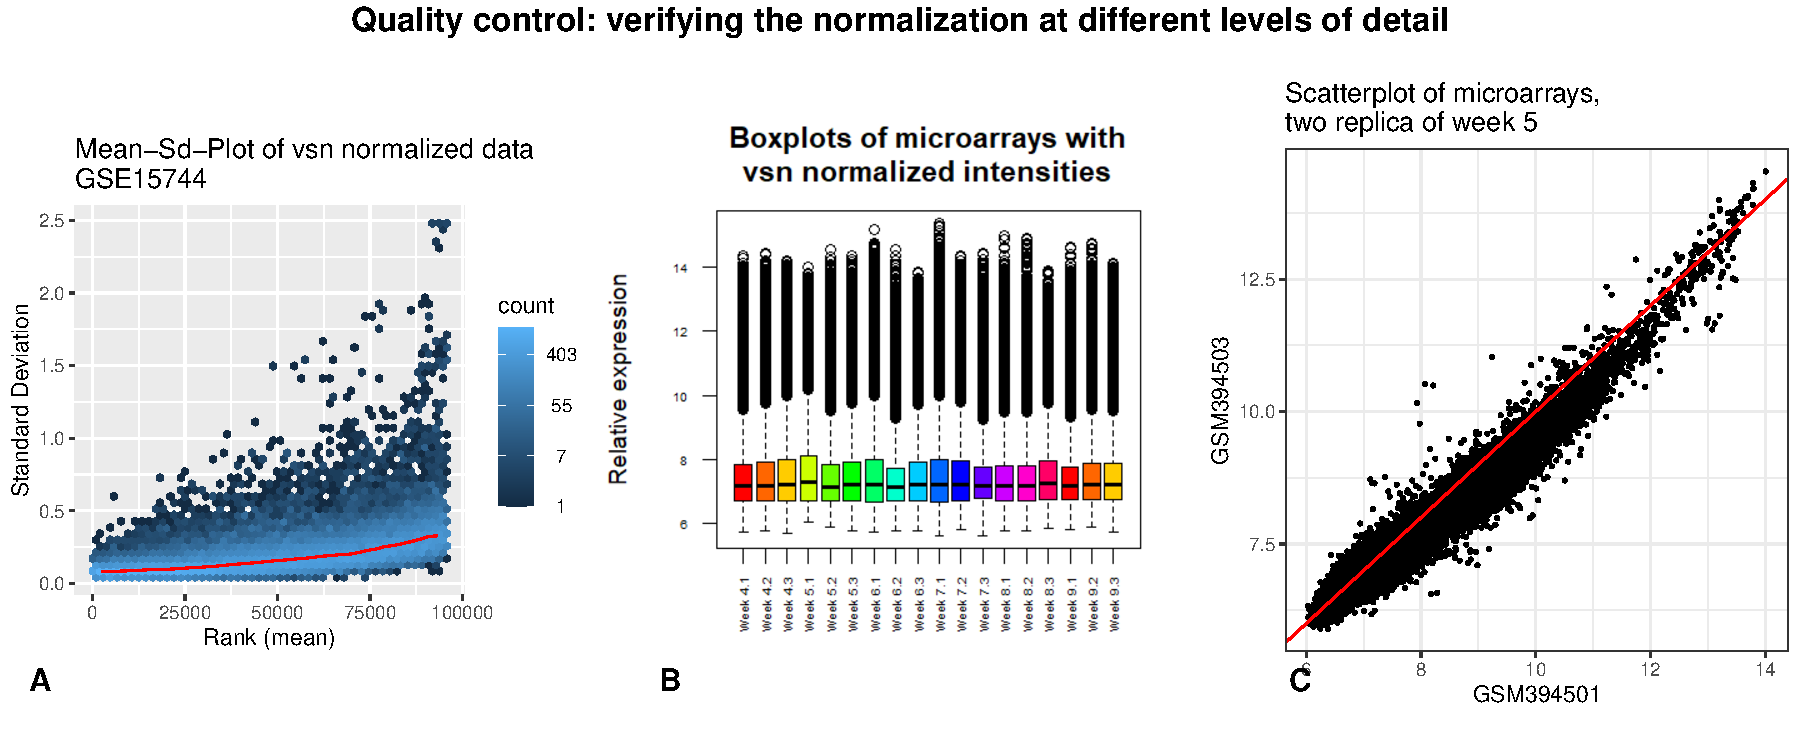
\includegraphics{final_report_files/figure-latex/QC-normalization-plots-1.pdf}
\caption{\label{fig:QC-normalization-plots}The plots support the use of the vsn normalization on our data set. A: The red line is close to horizontal, although it shows some correlation at high intensity leves. B: The boxplots show nice allignment of the mean intensity values. Some outliers are given but can neglected given the 0.25 and 0.75 quantile. C: A selected Scatterplot is shown. Very slight banana shaped structure can be seen, but only marginal. Overall the quality control confirmes successful vsn normalization}
\end{figure}

\hypertarget{differential-gene-expression---volcano-plot}{%
\subsection{Differential gene expression - Volcano Plot}\label{differential-gene-expression---volcano-plot}}

\begin{figure}
\centering
\includegraphics{final_report_files/figure-latex/Volcano-Plot-1.pdf}
\caption{\label{fig:Volcano-Plot}Volcanoplot for differential gene expression between week 4 and 9. The adjusted P-value boundary was set at 0.01. The logFC boundarys were -1 and 1.}
\end{figure}

\hypertarget{organ-development}{%
\subsection{Organ development}\label{organ-development}}

\begin{figure}
\centering
\includegraphics{final_report_files/figure-latex/tissue-links-1.pdf}
\caption{\label{fig:tissue-links}Each tissue is displayed as a node with its size representing the number of transcripts associated with it. The edges show the shared TRAs between the linked tissues, with only links corresponding to more than 100 common TRAs visible.}
\end{figure}

\begin{figure}
\centering
\includegraphics{final_report_files/figure-latex/heatmap-tissues-1.pdf}
\caption{\label{fig:heatmap-tissues}For each of the tissues on the right, the share of its TRAs that are also associated with the tissue in the respective column is displayed.}
\end{figure}

\begin{figure}
\centering
\includegraphics{final_report_files/figure-latex/spleen-boxplot-1.pdf}
\caption{\label{fig:spleen-boxplot}A further look on the expression of transcripts in the up- and downregulated clusters shows that the upregulated transcripts are close to the minimum expression level between 6 and 7 in week 4 and showing expressions between 7 and 8.5 by week 9. In contrast, the downregulated genes have very high expression levels (8-9) by week 4 and decrease to a more moderate expression between 7 and 8.5 analogous to the upregulated transcripts.}
\end{figure}

\begin{figure}
\centering
\includegraphics{final_report_files/figure-latex/spleen-down-table-1.pdf}
\caption{\label{fig:spleen-down-table}Table of all spleen-associated genes from the downregulated cluster with a function related to the cell cycle of cellular division}
\end{figure}

\begin{figure}
\centering
\includegraphics{final_report_files/figure-latex/spleen-up-table-1.pdf}
\caption{\label{fig:spleen-up-table}Table of all spleen-associated genes from the upregulated cluster with a function related to the spleens overall purpose (immune and blood-related genes)}
\end{figure}

\hypertarget{brain-development}{%
\subsection{Brain development}\label{brain-development}}

\begin{figure}
\centering
\includegraphics{final_report_files/figure-latex/boxplot-Cerebral-Hemisphere-1.pdf}
\caption{\label{fig:boxplot-Cerebral-Hemisphere}A boxplot of all Cerebellar Hemisphere genes was made to evaluate their scattering. For the samples of all weeks at the top and only for the three samples of week 4 on the bottom.}
\end{figure}

\begin{figure}
\centering
\includegraphics{final_report_files/figure-latex/Cerebellar-Hemisphere-specific-1.pdf}
\caption{\label{fig:Cerebellar-Hemisphere-specific}A boxplot of ENST00000276646, ENST00000518312 and ENST00000521485 was made to evaluate the scattering of the three samples per week for the 6 weeks from our dataset.}
\end{figure}

\end{document}
